\documentclass{article}
%% declare any packages used
\usepackage{graphicx}
\usepackage{natbib}
\usepackage{graphicx}
\usepackage{color} 
\usepackage{pdfpages}
\usepackage{appendix}
\usepackage{subfigure}
\usepackage{amsmath}
\usepackage{amssymb}


\begin{document}

\title{Supplementary material for referee\\MNRAS: MN-15-0213-MJ}
\maketitle

This is a supplementary documenting which presents a few plots to justify the claims made in the response to
referee for MNRAS submission MN-15-0213-MJ.

Figure 1 shows the level populations of Helium 1. Levels are split according to TopBase, meaning that they are in 
energy order and split by s and l quantum numbers.It demonstrates that in the dense regions of the wind in which He I emission tends to occur (Cell 10), the populations are already more or less distributed by statistical weight. The cells in the figure have the following properties:

\begin{itemize}
\item cell 10: $T_R=4.76e+04, T_e=3.43e+04, n_e=1.10e+14, W=3.49e-01$
\item cell 96: $T_R=4.69e+04, T_e=1.96e+04, n_e=5.26e+10, W=6.02e-03$
\item cell 200: $T_R=3.41e+04, T_e=1.49e+03, n_e=5.87e+07, W=1.41e-04$
\end{itemize}
Figure 2 shows a spectrum. One of the models has arbritrarily fast transitions added between forbidden transitions,
to simulate the effect of dominant collisional transitions between these states. The other model is model B from the 
paper, a model with significant He I emission. The effect on the overall spectrum is completely negligible. 

\begin{figure}	%fullpage
\centering
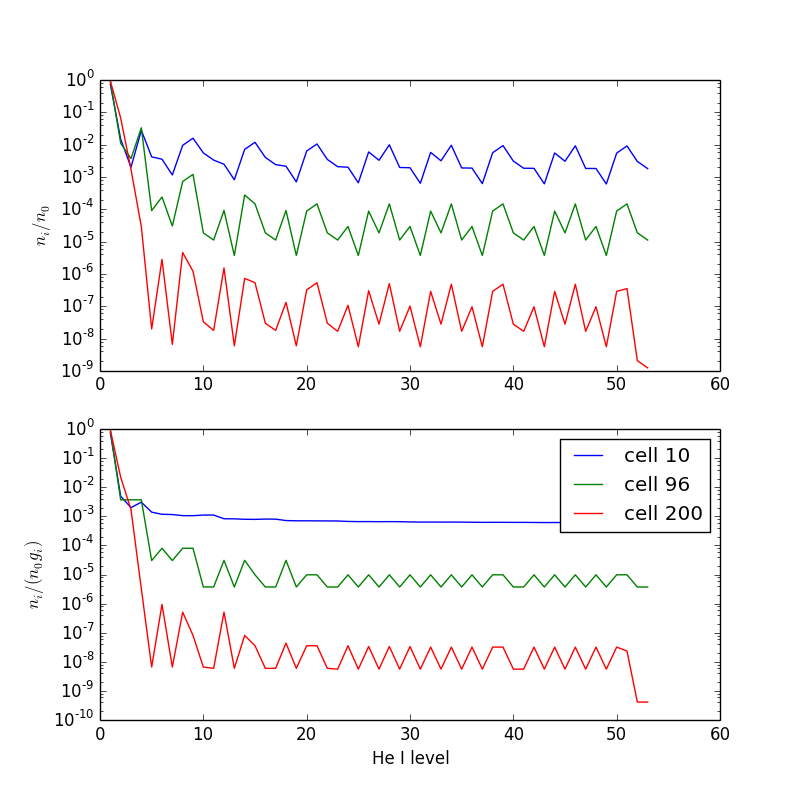
\includegraphics[width=1.0\textwidth]{pops.png}
\caption
{
Top Panel: fractional level populations in He I. Bottom Panel: fractional level populations in He I divided by statistical weight. In dense regions the levels are already distributed more or less according to statistical weight. This
is due to b-f processes dominating the level populations. As densities decrease, the triplet and singlet populations
become somewhat decoupled. This does not affect the model as these cells have negligible line emissivities.
}
\label{f1}
\end{figure}

\begin{figure}	%fullpage
\centering
\caption{
A spectrum will be shown here.
}
\label{f2}
\end{figure}

\end{document}
